% Author: Izaak Neutelings (April 2021)
\documentclass[border=3pt,tikz]{standalone}
\usepackage{physics}
\usepackage{tikz}
\usepackage[outline]{contour} % glow around text
\usetikzlibrary{calc}
\usetikzlibrary{angles,quotes,arrows.meta} % for pic
\usetikzlibrary{patterns}
\tikzset{>=latex} % for LaTeX arrow head
\contourlength{1.35pt}

\colorlet{xcol}{blue!70!black}
\colorlet{vcol}{green!60!black}
\colorlet{myred}{red!65!black}
\colorlet{mypurple}{blue!60!red!80}
\colorlet{acol}{red!50!blue!80!black!80}
\tikzstyle{rvec}=[->,xcol,very thick,line cap=round]
\tikzstyle{vvec}=[->,vcol,very thick,line cap=round]
\tikzstyle{mass}=[thin,draw=red!30!black, %rounded corners=1,
                  top color=red!40!black!30,bottom color=red!40!black!10,shading angle=30]
\tikzstyle{ground}=[preaction={fill,top color=black!10,bottom color=black!5,shading angle=20},
                    fill,pattern=north west lines,draw=none,minimum width=0.3,minimum height=0.6]
\tikzstyle{metal}=[fill,top color=black!40,bottom color=black!20,shading angle=10]


\begin{document}


% DISK
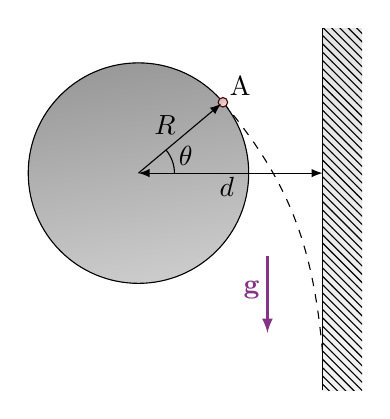
\begin{tikzpicture}
  \def\H{4.6}  % wall height
  \def\D{0.5}  % wall thickness
  \def\R{1.4}  % disk radius
  \def\r{0.06} % mass point radius
  \def\d{2.34} % wall's distances center
  \def\ang{40} % angle point 2
  \coordinate (O)  at (0,0);            % disk center
  \coordinate (W)  at (\d,-0.6*\H);     % wall bottom left
  \coordinate (WR) at (\d+\D,-0.6*\H);  % wall bottom right
  \coordinate (P)  at (\ang:\R);        % mass point
  \coordinate (P') at (\ang:\R-0.5*\r); % mass point
  \coordinate (L)  at (\d,-0.5*\H);     % land point
  \coordinate (R)  at (\R,0);           % disk right
  
  % GRAVITY
  \draw[->,acol,thick] (1.17*\R,-0.75*\R) --++ (0,-0.7*\R) node[pos=0.45,left=-1] {$\vb{g}$};
  
  % WALL
  \fill[ground]
    (W) rectangle++ (\D,\H);
  \draw (W) --++ (0,\H);
  
  % DISK
  \draw[dashed] (P) to[out=\ang-90,in=95] (L);
  \draw[metal] (O) circle(\R);
  \draw[mass] (P) circle(\r) node[above right=-1] {A};
  \draw[->] (O) -- (P') node[midway,above left=-2] {$R$};
  \draw[<->] (O) -- (\d,0) node[pos=0.48,below=-2] {$d$};
  \draw pic["$\theta$",draw=black,angle radius=13,angle eccentricity=1.4] {angle = R--O--P};
  
\end{tikzpicture}


\end{document}
